\section{Web}

The web part was developed in addition to the mandatory requirements. It runs through without the user having to do anything. 
For these reasons (especially the second one), the descriptions are also rather small. The code snippets here above show how a clean run without errors looks like.
In the web part, as in all other parts, everything necessary will be installed first.

\begin{lstlisting}
<INFO> - Tue Jan  8 11:24:21 UTC 2019 - Starting WEB Configurations.
<INFO> - Tue Jan  8 11:24:21 UTC 2019 - Will install 'nginx' now. Please wait...
...........
<INFO> - Tue Jan  8 11:24:32 UTC 2019 - Package 'nginx' is installed now.
<INFO> - Tue Jan  8 11:24:33 UTC 2019 - Will install 'certbot' now. Please wait...
....
<INFO> - Tue Jan  8 11:24:36 UTC 2019 - Package 'certbot' is installed now.
<INFO> - Tue Jan  8 11:24:36 UTC 2019 - Will install 'python-certbot-nginx' now. Please wait...
.......
<INFO> - Tue Jan  8 11:24:43 UTC 2019 - Package 'python-certbot-nginx' is installed now.
<INFO> - Tue Jan  8 11:24:43 UTC 2019 - Will install 'apache2' now. Please wait...
..............
<INFO> - Tue Jan  8 11:24:57 UTC 2019 - Package 'apache2' is installed now.
\end{lstlisting}



As the next step after installation, the nginix is configured.

\begin{lstlisting}
<INFO> - Tue Jan  8 11:24:57 UTC 2019 - Starting nginx Configurations.
<INFO> - Tue Jan  8 11:24:57 UTC 2019 - Nginx is already activated.
<INFO> - Tue Jan  8 11:24:57 UTC 2019 - Start Nginx Hardening. (TLS, redirect http->https, secuirty headers, no server token, timeouts)
\end{lstlisting}

With openssl a certificate will be created in a next step. The certificate is then used for ssl termination.

\begin{lstlisting}
<INFO> - Tue Jan  8 11:24:57 UTC 2019 - Start openssl to generate a ssl pem file.
Generating DSA parameters, 4096 bit long prime
.............+.......+.....+.........+..............
+++++++++++++++++++++++++++++++++++++++++++++++++++*
.............+..+.+.................+.....+...+.....
.........+......+.......+...........................
<INFO> - Tue Jan  8 11:25:08 UTC 2019 - Done. Your file is located here: /etc/ssl/dh4096.pem. Will start certbot.
Saving debug log to /var/log/letsencrypt/letsencrypt.log
Plugins selected: Authenticator nginx, Installer nginx
Obtaining a new certificate
Performing the following challenges:
http-01 challenge for examplerun.cf
http-01 challenge for www.examplerun.cf
Waiting for verification...
Cleaning up challenges

IMPORTANT NOTES:
- Congratulations! Your certificate and chain have been saved at:
/etc/letsencrypt/live/examplerun.cf/fullchain.pem
Your key file has been saved at:
/etc/letsencrypt/live/examplerun.cf/privkey.pem
Your cert will expire on 2019-04-08. To obtain a new or tweaked
version of this certificate in the future, simply run certbot
again. To non-interactively renew *all* of your certificates, run
"certbot renew"
- If you like Certbot, please consider supporting our work by:

Donating to ISRG / Lets Encrypt:   https://letsencrypt.org/donate
Donating to EFF:                    https://eff.org/donate-le
\end{lstlisting}

Nginx will then be hardened:
\begin{itemize}
    \item{Enable secure SSL protocols only (>=TLSv1.2)}
    \item{Secure cipher sets (no known vulnerabilities)}
    \item{Redirect all connections from HTTP to HTTPS}
    \item{Turn off server tokens}
\end{itemize}

\begin{lstlisting}
<INFO> - Tue Jan  8 11:25:19 UTC 2019 - Will remove default sites of nginx
<INFO> - Tue Jan  8 11:25:19 UTC 2019 - Will start to setup nginx.conf file
<INFO> - Tue Jan  8 11:25:19 UTC 2019 - Done. Your file is located under '/etc/nginx/nginx.conf'.
<INFO> - Tue Jan  8 11:25:19 UTC 2019 - Will start specific Configurations
<INFO> - Tue Jan  8 11:25:19 UTC 2019 - Done. Your file is located under '/etc/nginx/conf.d/examplerun.cf.conf'.
<INFO> - Tue Jan  8 11:25:19 UTC 2019 - Will check Syntax and activate.
nginx: the configuration file /etc/nginx/nginx.conf syntax is ok
nginx: configuration file /etc/nginx/nginx.conf test is successful
\end{lstlisting}

In the next and last step the apache will be configured. This setup places apache behind nginx as pure webserver.
All connections are passed through nginx where SSL is terminated. Later on it would be possible to extend this setup with a \gls{WAF} like \gls{ModSecurity} which would provide an aditional security layer. See section \ref{more_hardening}.
\begin{lstlisting}
<INFO> - Tue Jan  8 11:25:19 UTC 2019 - Starting apache Configurations.
<INFO> - Tue Jan  8 11:25:19 UTC 2019 - Apache is already activated.
<INFO> - Tue Jan  8 11:25:19 UTC 2019 - Found enabled default site, removing symlink
<INFO> - Tue Jan  8 11:25:19 UTC 2019 - Will Setup a default mini webpage.
<INFO> - Tue Jan  8 11:25:19 UTC 2019 - Will Setup a seperate ports.conf file.
<INFO> - Tue Jan  8 11:25:19 UTC 2019 - Will Setup avaible sites.
<INFO> - Tue Jan  8 11:25:19 UTC 2019 - Will check Syntax and activate.
Syntax OK
\end{lstlisting}

\subsection{Web architecture diagram}
For a better understanding of how the proxy server interacts with the web server, see this small diagram.
\begin{figure}[H]
	\centering
	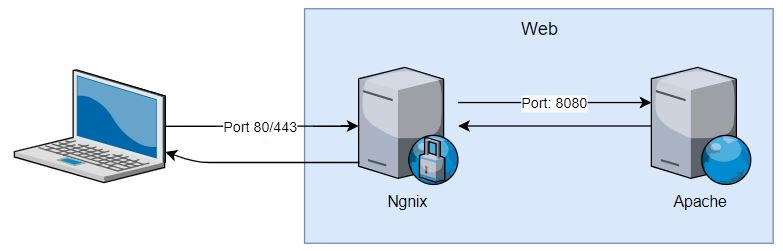
\includegraphics[width=0.9\linewidth]{diagram/web_arch_diagramm.JPG}
	\caption{Architecture Web}
	\label{fig:beforeWeb}
\end{figure}
